\documentclass[usegeometry=true]{scrartcl}
\usepackage[ngerman]{babel}
\usepackage[T1]{fontenc}
\usepackage{lmodern}
\usepackage[utf8]{inputenc}
\usepackage{hyperref}
\usepackage{amssymb}
\usepackage{graphicx}
% Dimensionen bitte nicht ändern. 
\usepackage[left=2cm, right=2cm, top=2cm, bottom=2cm, bindingoffset=1cm, includeheadfoot]{geometry}
%Zeilenabstand bitte nicht ändern
\usepackage[onehalfspacing]{setspace}

\bibliographystyle{unsrt}

\begin{document}
% ----------------------------------------------------------------------------
\subject{Projektbericht zum Modul Information Retrieval und Visualisierung Sommersemester 2021}
\title{Bike Buyers 1000}
%\subtitle{Untertitel}% optional
\author{Floyd Spuhler}% obligatorisch
\date{10.9.2021}
\maketitle% verwendet die zuvor gemachte Angaben zur Gestaltung eines Titels
% ----------------------------------------------------------------------------
% Inhaltsverzeichnis:
%\tableofcontents
% ----------------------------------------------------------------------------
% Gliederung und Text:

\section{Einleitung}
Tipps zu Latex und Koma-Script für Hausarbeiten sind im \href{http://mirrors.ctan.org/info/latex-refsheet/LaTeX_RefSheet.pdf}{LaTeX Reference Sheet for a thesis with KOMA-Script} von Marion Lammarsch und Elke Schubert zusammengefasst. 
Der Bericht fällt in die Kategorie von InfoVis-Paper, die Tamara Munzner Design Study nennt \cite{Munzner2008}: In der Einleitung sollen sie zuerst das Zielproblem beschrieben. Daraus sollen sie Fragestellungen motivieren, die mittels Techniken der Informationsvisualisierung beantwortet werden können. \newline
\newline Fragestellungen: Welche Eigenschaften lasssen sich aus den Bike-Buyers-Daten ableiten? Darstellungen: Scatterplot, Parallele Koordinaten

\subsection{Anwendungshintergrund}
Sie müssen genug Hintergrund bereitstellen, so dass die Lesenden sich ein Urteil bilden können, ob ihre Lösung funktioniert. Sie sollen die Lesenden jedoch nicht mit Anwendungsdetails so überschütten, dass der Fokus auf die Fragen zur Informationsvisualisierung untergehen. \cite{Platter.2020}

Anwendungshintergrund: Diese Forschunngsarbeit bereitet Informationen auf, die Interessante Einblicke in das Kaufverhalten von Fahrrad-Kunden geben. So laassen sich anhand von einkommensdaten, dem Alter und dem Bildungshintergrund \cite{Munzner.2008} g 
\cite{Platter.2020}
\subsection{Zielgruppen}
Beschreiben sie die Personengruppe oder Personengruppen, die das von ihnen benannte Anwendungsproblem lösen möchte. Auf welches Vorwissen können sie in dieser Gruppen von Anwenderinnen aufbauen? Welche Informations"-bedürf"-nisse werden durch die Visualisierungen adressiert?
Dieser Forschungsbericht richtet sich vor allem an die Anbieterseite auf den B2C Fahrradmarkt. Hierzu lassen sich verschiedene Untergruppen kategorisieren.
 
Für Fahrradhersteller sind Informationen zum Alter der Kundengruppe für Rahmengröße, Fahrradart, sowie zum EInkommen in Hinblick auf die Auswahl der Materialenund deren Qualität wichtig. 

Für Fahrradverkäufer spielt vor allem der Verwendungszweck des potenziellen Kunden eine übergreordete Rolle beim Fahrradkauf. Die Wahl des richtigen Modells unterscheidet sich für die Freizeit (Mountainbike) mit weiten Distanzen vom Gebrauch für die Stadt mit geringeren Distanzen (Stadtrad). 

Auch für Unternehemn aus der Baubranche mit dem Fokus auf die Infrastruktur für Fahrradwege ist diese Arbeit eine geeignete Anslaufstelle für Informationen zum Einsatz des Fahrrads in Bezug auf den Arbeitsweg. 


\paragraph{Zielgruppe:}Fahrradunternehmen mit Interesse zur Preisbildung, Marktsegmentierung -> Kundenakquise, 
\subsection{Überblick und Beiträge}
In diesem Abschnitt geben sie einen kurzen Überblick über die Daten und verwendeten Visualisierungen. Dann benennen sie die Beiträge ihres Projekts. Diese Beiträge müssen sie in den hinteren Teilen des Berichts genauer ausführen und belegen.
\paragraph{Überblick:}
Die durch Kaggle bereitgestellten Daten bestehen aus demographischen Kundeninformationen, wie Alter, Geschlecht, Familienstand etc. Diese Daten werden in drei visualiserungen dargestellt, um Herstelleranalysten einen Überblick in diese Kundendaten zu vermitteln.

\section{Daten}
Beschreiben Sie vorhandenen Daten. Gehen sie kritisch darauf ein, in wie weit sich die Daten für die Bearbeitung der Fragestellungen und dem Erreichen von Lösungen für die oben beschriebene Zielgruppen eignen. Haben sie die Daten sinnvoll mit weiteren Datenquellen ergänzt? Wenn ja, wie?

Die diesem Projektbericht zugrundeliegenden Rohdaten entstammen einem Datensatz des " Kaggle" -Account von Heeral Dedhia, welche Antworten von 1.000 NutzerInnen zum Thema Fahrradkauf bereitstellt. Die Nutzerin hat diese Daten zuletzt im Jahresverlauf 2020 erweitert. Datum- und Erhebungsform sind hierbei unbekannt. In dieser aktuellsten Version liegen 13 verschiedene Attribute zu den 1000 befragten Personen vor. Die Nutzerin hat zwei verschiedene Datensätze bereitgestellt, die sich lediglich durch NA-Werte unterscheiden. Zu Übersichtszwecken stellt die bereinigte Datei "bikebuyersclean.csv" die Grundlage für dieses Visualisierungsprojekt dar (ToDo: Kaggle Seite zitieren). 

zu allen befragten personen wurde eine eindeugige ID vergeben, welche ein INT-Typ ist. Zur quantifizierung der Baumhierarchie wurde diese Tabellenspalte für die dritte Visualiserung übernommen. Die nächsten beiden Spalten "Marital Status" , "Gender" und "Children" und "Age" als Int geben als String-Datentyp Aufschluss über den sozialen  Familienstand und Geschlecht der befragten Person. Die Spalten "Income", "Education" , "Occupation" geben Auffschluss über die berufliche Karriere. In Verbindung mit den Spalten "HomeOwner" und "Cars" lässt sich der Status der Person interpretieren. Das Attribut "Commute Distance" gibt Aufschluss über die Distanz zur Arbeit" dient der Befragung zur Entfernung zwischen Wohnort und Arbeitsstätte, wodurch wertvolle Informationen zwischen Cars, Bikes und co gewonnen werden können. Durch purchasedBike und Region können diese Daten weiter voneinander unterschieden oder für einen globalen Einblcik als ganzes betrachtet werden. 

Die Daten eignen sich besonders für Analysten von Fahrradunternehmen, die beispielsweise einen Online-Fahhrad-Shop betreiben wollen. Hierdurch erhalten sie eine Grundlage über mögliche Kundengruppen, wodurch wertvolle Informationen, wie die Arbeitsentferung vorhanden sind und sich insbesondere in der zukünftigen Infrastruktur von Großstädten bemerkbar machen werden. Auch in Hinblick auf die anhaltende covid-19 Krise und den sicheren Aspekt des Individualverkehrs bietet eiun Fahrad auf kurze bis mittlere Distanz eine umweltschonende und kostengünstige Alternative zum Auto. 
Diese Informationen in Verbindlung mit dem Alter, Einkommen und Beruf können individuelle Kundengruppen angesprochen werden. 

Um eine geeignete Überblicksmöglichkeit über diese potenziellen Kundengruppen zu schaffen, musste der dafür notwendige Datensatz für die Baumhierarchie angepasst werden. 

\subsection{Technische Bereitstellung der Daten}
Wie sind die Daten zugänglich? Welche Formate werden genutzt. Gibt es Besonderheiten beim Lesen der Formate?



Der zugrundeliegende Datensatz wurde um keine zusätzlichen Daten erweitert. Die Daten bilden eine gute Verteilung in verschiedenen Regionen ab, sind ausgewogen verteilt und bieten eine vielzahl an Informationen, mit denen Fahrradhersteller / Verkäufer wie Onlineshiops gezielt Kundengruppen ansprechen können. 
\subsection{Datenvorverarbeitung}
Welche Datenvorverarbeitungsschritte sind notwendig? Beschreiben Sie die einzelnen Schritte und begründen sie sie, z.B. warum werden manche Daten weggelassen, über welche Mengen werden Durchschnitte berechnet, warum sind die so berechneten Werte aussagekräftiger als andere Werte. 

\paragraph{Vorverarbeitung:} Die Vorverarbeitung erfolgt im filtern leerer Felder

\section{Visualisierungen}
\subsection{Analyse der Anwendungsaufgaben}
Analysieren sie die konkreten Anwendungsaufgaben. Welche Visualisierungen helfen den Personen, die die Software verwenden, sinnvolle mentale Modelle aufzubauen. Sind diese mentalen Modelle für sie notwendig, um die Aufgaben lösen zu können?
\subsection{Anforderungen an die Visualisierungen}
Leiten sie Anforderungen an das Design der Visualisierungen ab, die sich durch ihre Analyse des Zielproblems ergeben.
\subsection{Präsentation der Visualisierungen}
Präsentieren sie die visuelle Abbildungen und Kodierungen der Daten und Interaktionsmöglichkeiten. 
Sie müssen  begründen, warum und wiegut ihre Designentscheidungen die erstellten Anforderungen erfüllen. 
Weiterhin müssen sie begründen, warum die gewählte visuelle Kodierung der Daten für das zulösenden Problem passend ist. 
Typische Argumente würden hier auf Wahrnehmungsprinzipien und Theorie über Informationsvisualisierung verweisen. 
Die besten Begründungen diskutieren explizit die konkrete Auswahl der Visualisierungen im Kontext von mehreren verschiedenen Alternativen. Diskutieren sie die Expressivität und die Effektivität der einzelnen Visualisierungen. 

Die eben beschriebenen Präsentationen und Begründungen sollen für jede der drei folgenden Visualisierungen durchgeführt werden. 
\subsubsection{Visualisierung Eins}



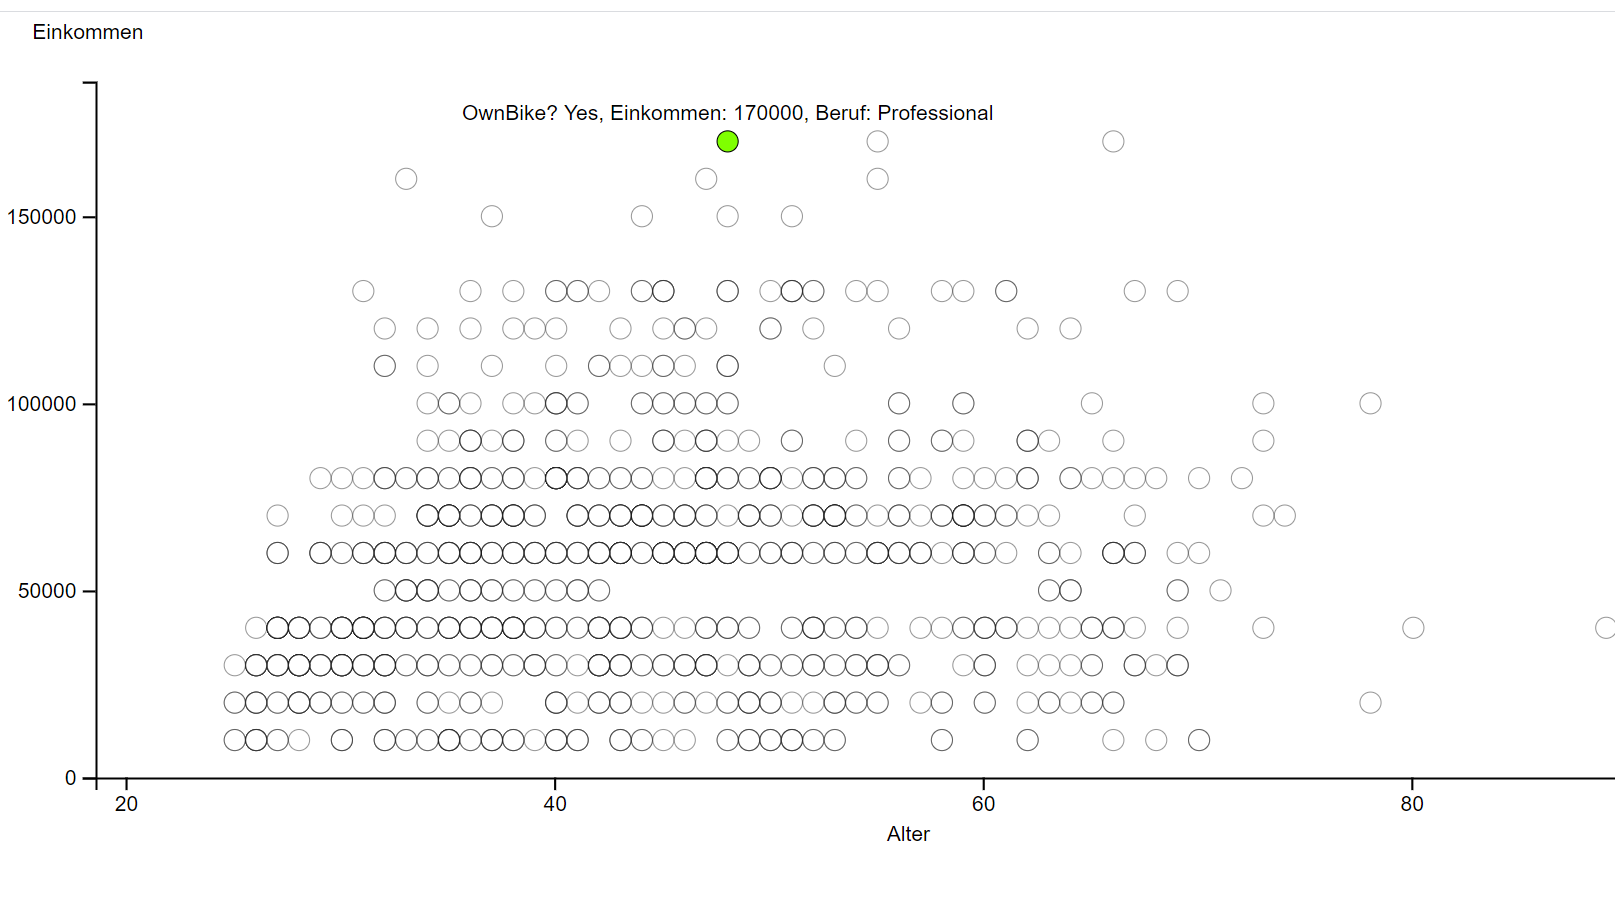
\includegraphics{Scatterplot1}

\subsubsection{Visualisierung Zwei}

TestText 123

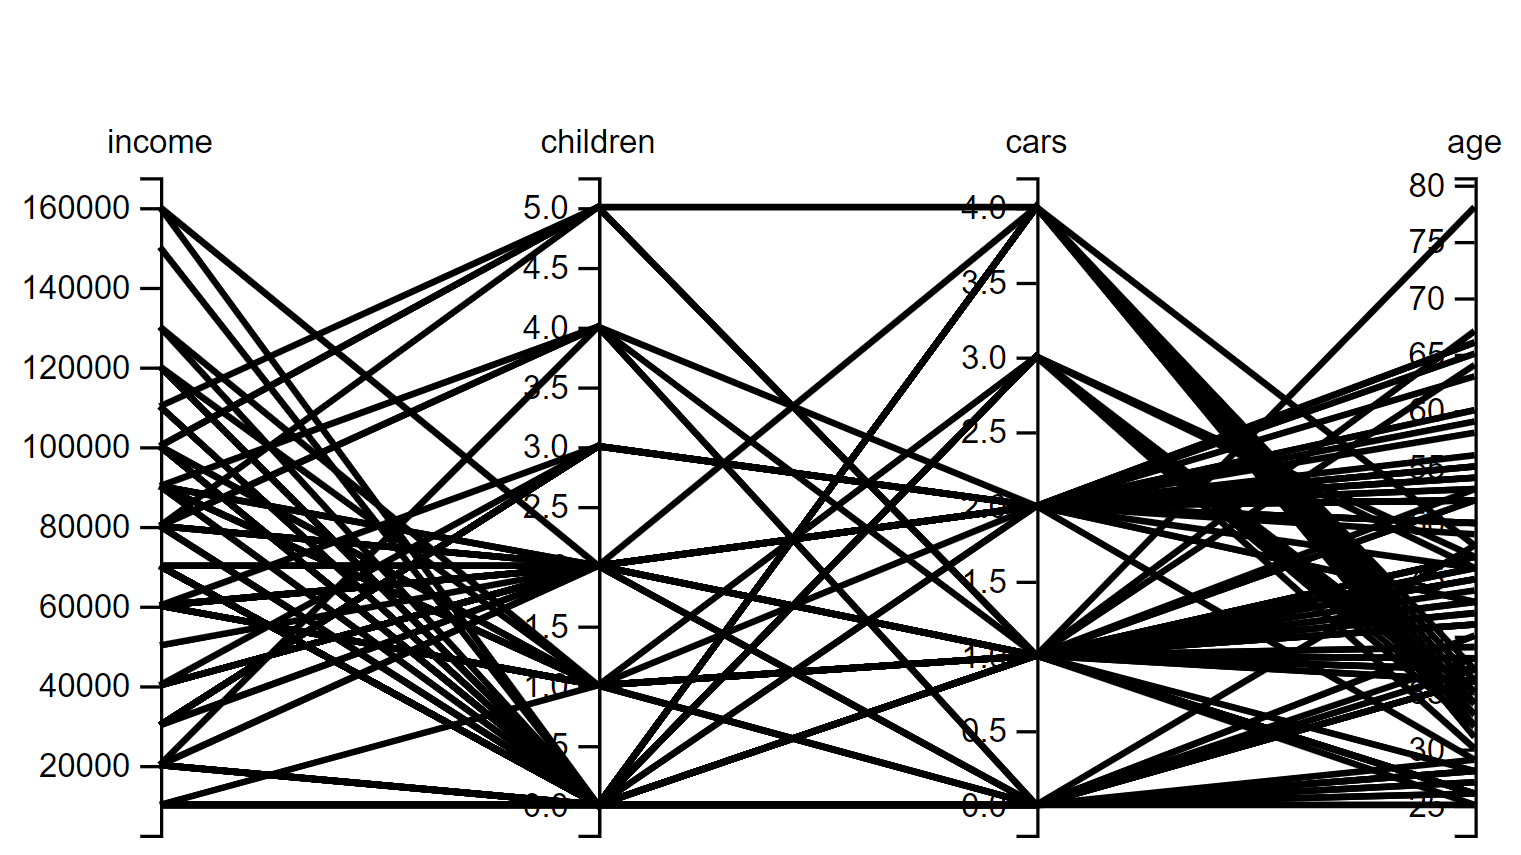
\includegraphics{parallelcoordinates}

TestText 123
\subsubsection{Visualisierung Drei}

\subsection{Interaktion}
Erklären sie die möglichen Interaktionen mit den einzelnen Visualisierungen und die möglichen Verknüpfungen zwischen ihnen. Begründen Sie warum die konkreten Interaktionen umgesetzt wurden und welche Zwecke für die Anwenderinnen mit ihnen unterstützt werden. Begründen sie ebenfalls warum sie andere Interaktionsmöglichkeiten nicht umgesetzt haben. 

\section{Implementierung}
Beschreiben Sie die Implementierung ihrer Visualisierungsanwendung in Elm. Stellen die Gliederung ihres Quellcodes vor. Haben Sie verschiedene Elm-Module erstellt. Was war aufwändig umzusetzen, was ließ sich mit dem vorhanden Code aus den Übungen relativ einfach umsetzen? 

Wie sieht die Elm-Datenstruktur für das Model aus, in dem die verschiedenen Zustände der Interaktion gespeichert werden können.

\section{Anwendungsfälle}
Präsentieren sie für jede der drei Visualisierungen einen sinnvollen Anwendungsfall in dem ein bestimmter Fakt, ein Muster oder die Abwesenheit eines Musters visuell festgestellt wird. Begründen sie warum dieser Anwendungsfall wichtig für die Zielgruppe der Anwenderinnen ist. Diskutieren sie weiterhin, ob die oben beschriebene Information auch mit anderen Visualisierungstechniken hätte gefunden werden können. Falls dies möglich wäre, vergleichen sie die den Aufwand und die Schwierigkeiten ihres Ansatzes und der Alternativen. 
\subsection{Anwendung Visualisierung Eins}
\subsection{Anwendung Visualisierung Zwei}
\subsection{Anwendung Visualisierung Drei}

\section{Verwandte Arbeiten}
Führen sie eine kurze Literatursuche in der wissenschaftlichen Literatur zu Informationsvisualisierung und Visual Analytics nach ähnlichen Anwendungen durch. Diskutieren sie mindestens zwei Artikel. Stellen sie Gemeinsamkeiten und Unterschiede dar.

\section{Zusammenfassung und Ausblick}
Fassen sie die Beiträge ihre Visualisierungsanwendung zusammen. Wo bietet sie für die Personen der Zielgruppe einen echten Mehrwert.

Was wären mögliche sinnvolle Erweiterungen, entweder auf der Ebene der Visualisierungen und/oder auf der Datenebene?

\section*{Anhang: Git-Historie}
\newpage
\bibliography{literatur}


\end{document}

